\documentclass[a4paper, 10pt]{report}
\usepackage[italian]{babel}
\usepackage[T1]{fontenc}
\usepackage[utf8]{inputenc}
\usepackage{charter}
\usepackage{amsmath}
\usepackage{amsthm}
\usepackage{amsfonts}
\usepackage{graphicx}
\usepackage{wrapfig}
\usepackage{tcolorbox}
\usepackage{fancyhdr}
\usepackage{longtable}

\usepackage{geometry}
\geometry{a4paper, left=2cm,right=2cm,top=2cm,bottom=2cm}

\pagestyle{fancy}
\chead{}
\rhead{\bfseries 21 ottobre 2019}
\lhead{\bfseries Basi di dati}

\begin{document}
\begin{longtable}{| p{.16\textwidth} | p{.79\textwidth} |}
\textbf{Generalizzazione} & Una generalizzazione rappresenta un legame (simile all'ereditarierà delle classi) tra un'entità padre $E$ ed $n > 0$ entità figlie $E_1,...,E_n$, dove l'entità padre $E$ rappresenta una classe di oggetti più grande rispetto alle classi di oggetti rappresentate dalle entità figlie $E_1,...,E_n$.

Si rappresentano come segue:

\begin{center}
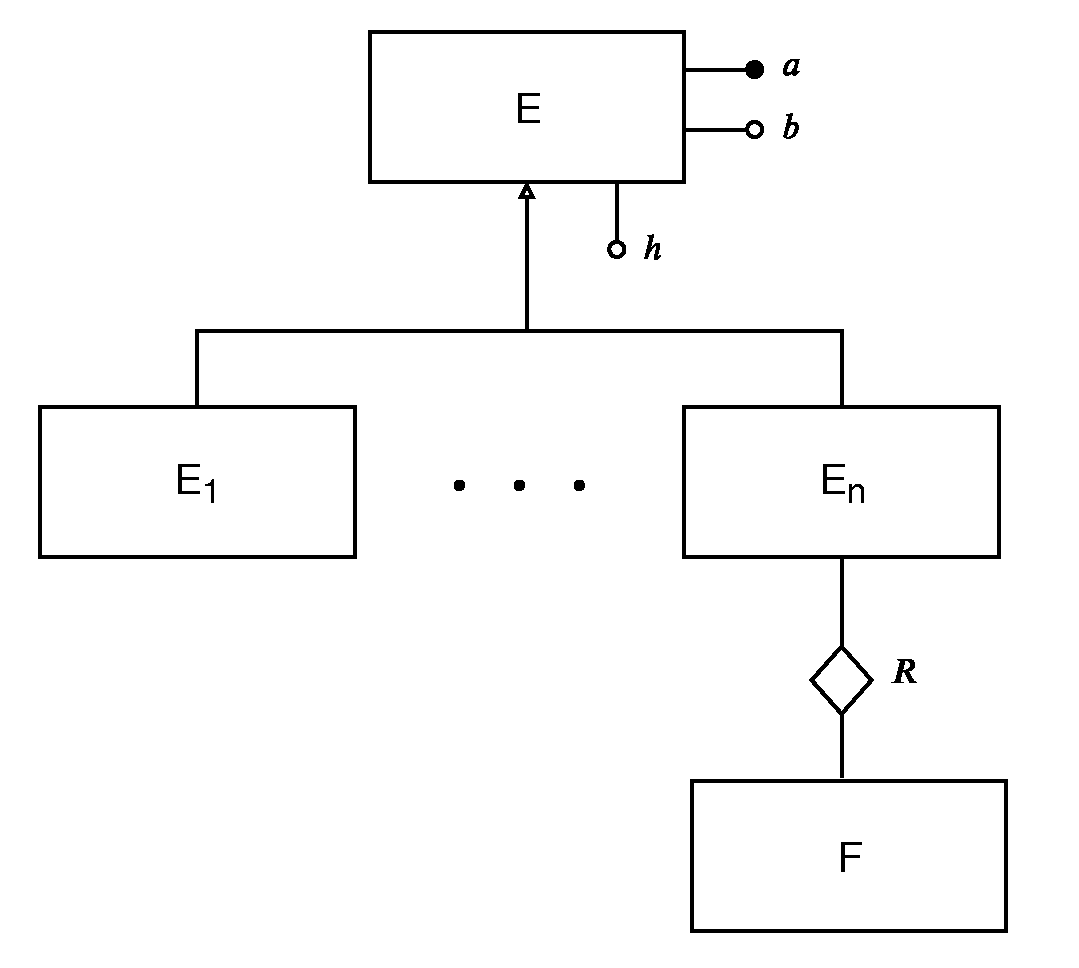
\includegraphics[scale=0.4]{21ottobre01.pdf}
\end{center}

Proprietà delle generalizzazioni:
\begin{itemize}
\item[-] Ogni istanza delle entità figlie $E_1,...,E_n$ è anche istanza dell'entità padre $E$ (condivisione di istanza tra la popolazione delle entità);
\item[-] Tutte le proprietà (attributi, relazioni e identificatore) delle istanze dell'entità padre $E$ sono anche proprietà delle istanze delle entità figlie $E_1,...,E_n$.  
\end{itemize}

\begin{center}
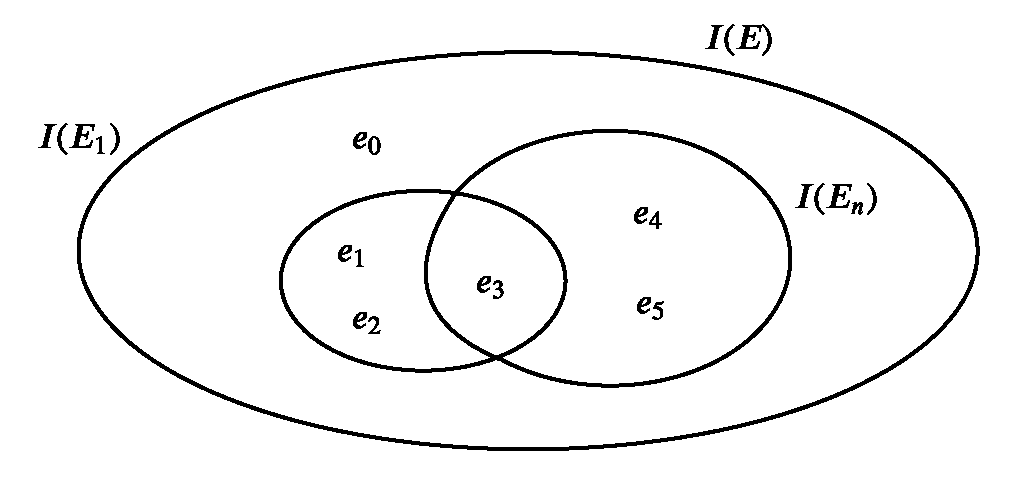
\includegraphics[scale=0.4]{21ottobre02.pdf}

(Rappresentazione insiemistica -> le istanze di $E$ sono date da quelle di $E$ + quelle delle figlie)
\end{center}


\underline{Esempio}:

\begin{center}
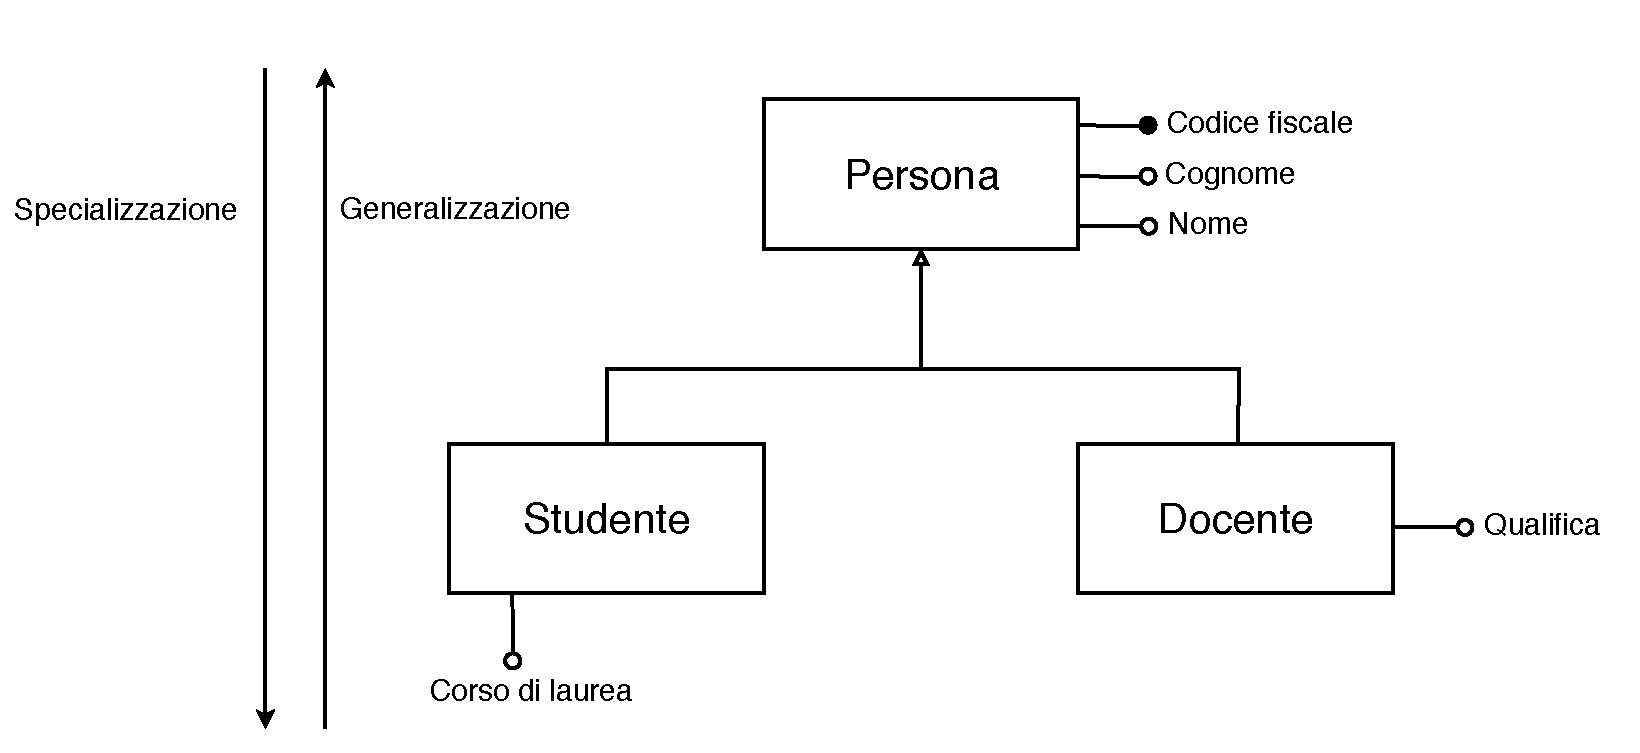
\includegraphics[scale=0.4]{3.pdf}
\end{center}

\end{longtable}

\begin{longtable}{| p{.16\textwidth} | p{.79\textwidth} |}
 & Classificazione delle generalizzazioni:
\begin{itemize}
\item[-] Una generalizzazione di dice totale se ogni istanza del padre $E$ è anche istanza di almeno una entità figlia $E_1,...,E_n$.

Una generalizzazione non totale si dice parziale;
\item[-] Una generalizzazione si dice esclusiva se ogni istanza delle entità figlie appartiene al massimo ad una sola entità figlia $E_i$.
\end{itemize}

Una generalizzazione non esclusiva si dice sovrapponibile.
 
\begin{center}
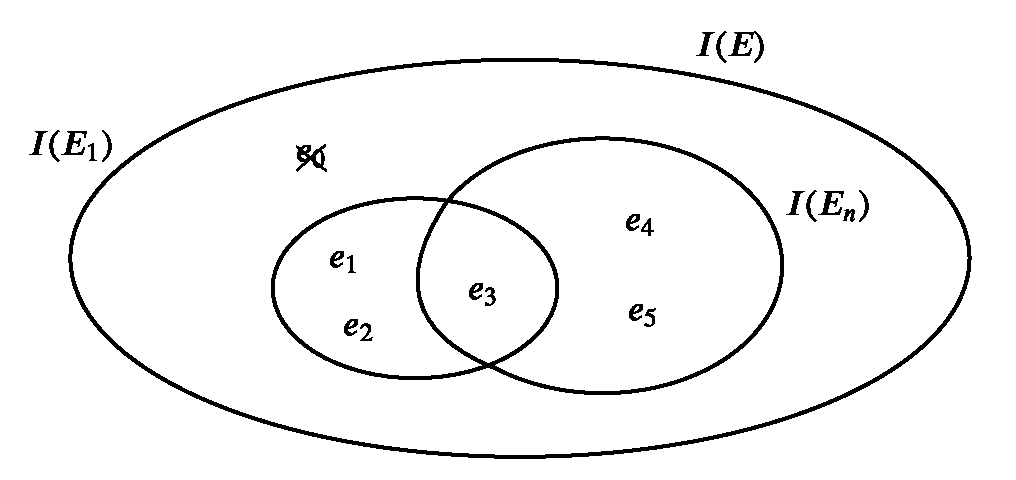
\includegraphics[scale=0.35]{21ottobre04.pdf}

(Totale)

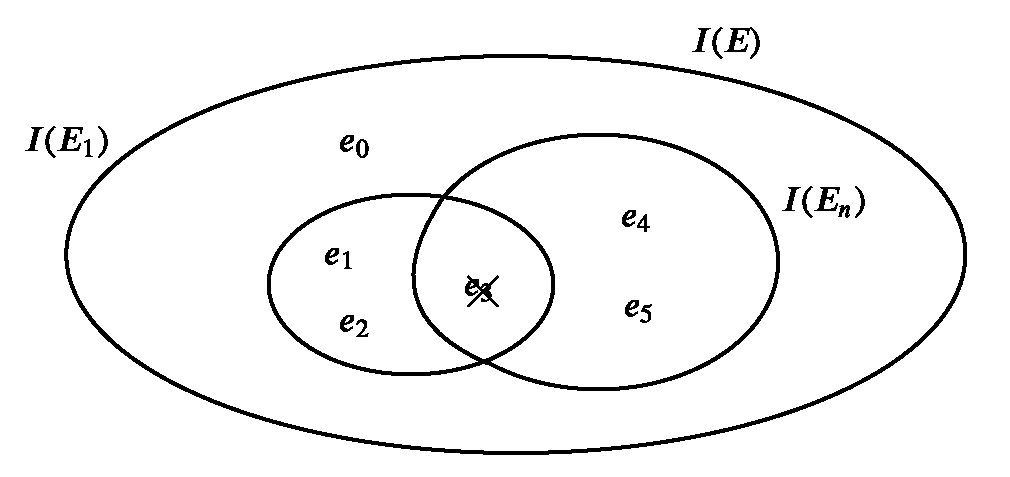
\includegraphics[scale=0.35]{21ottobre05.pdf}

(Esclusiva)
\end{center}

La classisificazione viene rappresentata come segue:



\begin{itemize}
\item[-] $(t, e)$ -> totale esclusivo;
\item[-] $(p, e)$ -> parziale esclusivo;
\item[-] $(t, s)$ -> totale sovrapposto;
\item[-] $(p, e)$ -> parziale sovrapposto (valore di default, non si indica);
\end{itemize}

\begin{center}
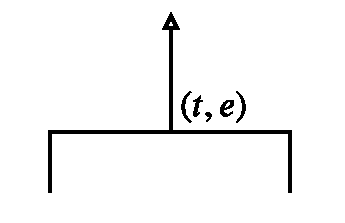
\includegraphics[scale=0.6]{21ottobre06.pdf}
\end{center}
\end{longtable}

\subsubsection*{Esercizio ER2}

\begin{center}
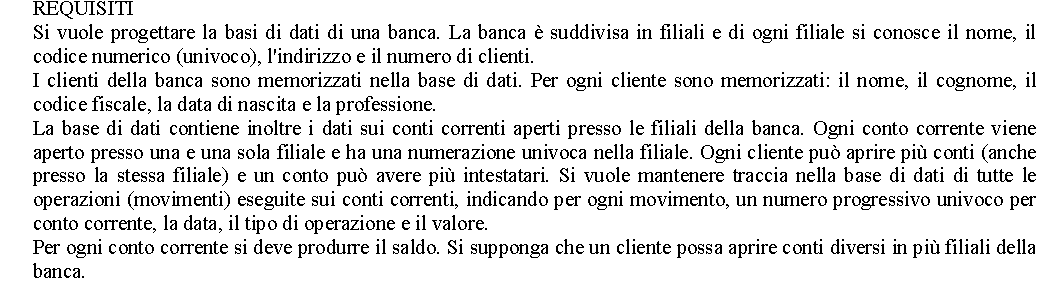
\includegraphics[scale=1.0]{er2.pdf}

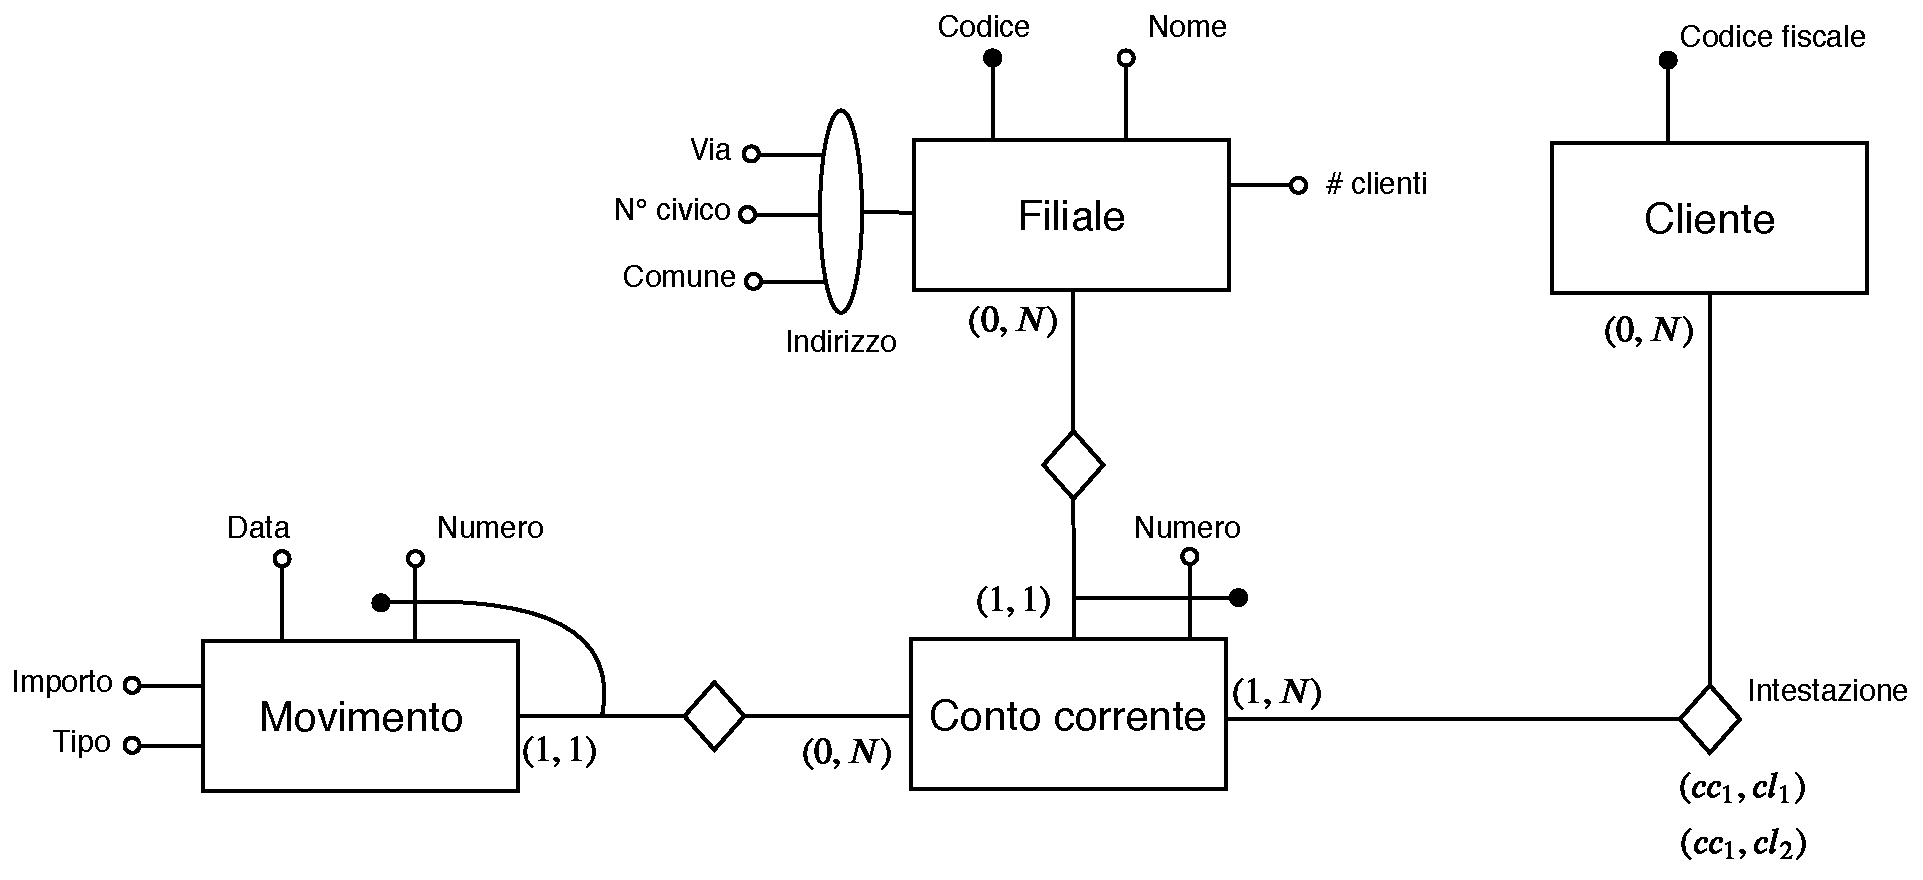
\includegraphics[scale=0.5]{21ottobre10.pdf}
\end{center}

\subsection*{Approfondimento sulle relazioni ternarie}

\begin{center}
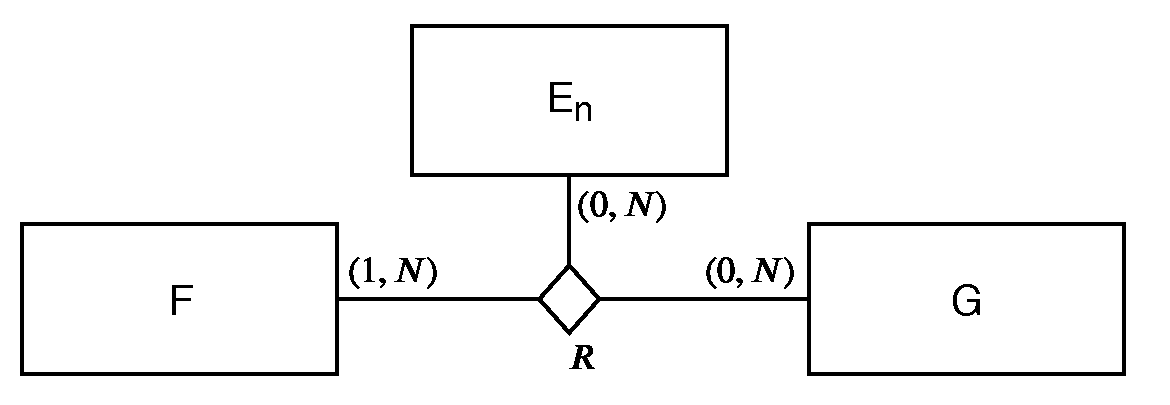
\includegraphics[scale=0.5]{21ottobre08.pdf}

($I(R) = \{(e_1, g_1, f_1)$)
\end{center}

\noindent Difficilmente si hanno vincoli di cardinalità diversi da $(0, N)$ e $(1, N)$; i vincoli di cardinalità non hanno impatto sull'istanziazione della relazione\footnote{se ho $0$
come $min$, vuol dire che posso avere delle istanze di $E$ che possono essere esterne alla relazione, In ogni caso la relazione, per esistere, deve avere un'istanza di tutti i "tipi necessari"}. \\

\paragraph*{Trasformazione da ternaria a doppia binaria} É possibile trasformare una relazione ternaria in una coppia di relazioni binarie?

  \begin{center}
    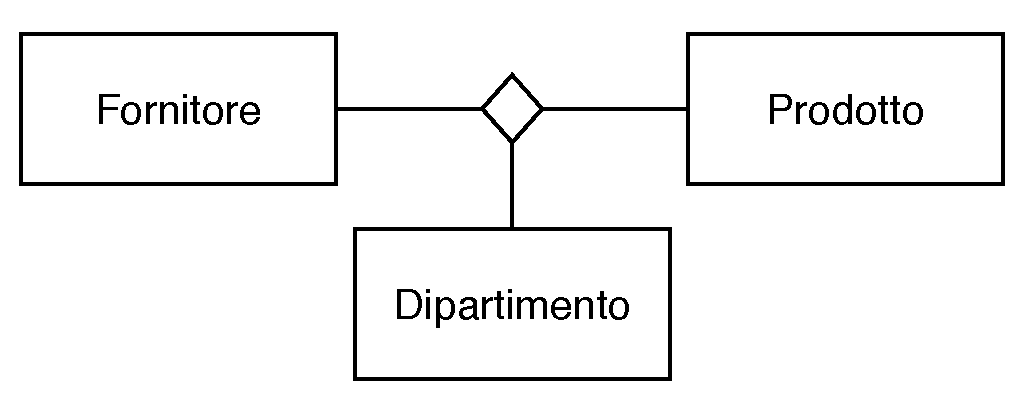
\includegraphics[scale=0.5]{21ottobre09.pdf}
    
    
I(fornitura) = \{

(d1, f1, p1), 

(d2, f1, p3), 

(d1, f3, p3), 

(d2, f3, p2), 

...
\}
  \end{center}





\end{document}
